
\chapter{Conditional random field}
Graphical models allow us to encode relationships between multiple variables using a concise, well-defined language. Because it's hard to solve the problems deterministically in real world. \textit{Probabilistic graphical model}(PGM)\cite{koller2009probabilistic} can assist in this case by encoding a joint or conditional probability distribution with graph, which means that PGM can encode the relationships between multiple random variables. 

The various types of PGM differ by the graph structure and the conditional independence assumptions. There are mainly two types, directed and undirected graph. Directed graphical model which is also called Bayesian network, specifies the family of distributions by means of directed acyclic graph and its joint distribution is factorized over each node which is a random variable with probability distribution conditioned on its parents. On the other hand, undirected graphical model, also known as Markov random field has undirected acyclic or cyclic graph. Its joint distribution is factorized over cliques, which is a fully-connected subgraph within the graph. This means, the marginal probability distribution in undirected graphical model is not normalized over nodes, but over cliques. 

In a object recognition task, the input is set of images and output is set of predicted labels. Because the dimensionality of input is always large so that it's difficult to model it directly. Nevertheless, we want to exploit the contextual relationship between different objects. To this end, it's better to just model the relationship between output random variables, which obey the conditional distribution of output given input. \textit{Conditional random field}(CRF), first proposed by \cite{lafferty2001conditional}, is a suitable model for this purpose. In this chapter, a concise introduction of CRF is given, including definition, learning and inference in the following subsection.
 
\section{Definition}
CRF can model the conditional distribution of a set of output random variables $\bld y$ given a set of inputs $\bld x$, that is $p(\bld y | \bld x)$. In the scope of scene object recognition problem, assume we have multiple objects in one scene denoted by $\bld x = [x_1, ..., x_n]$ and their labels $\bld y = [y_1, ..., y_n]$. We want to learn $p(\bld y | \bld x)$ with CRF and make predictions for unseen data.  

To formulate the problem clearly, we denote the set of output random variables by $\bld y$ and overall output domain by $\mathcal{Y}$. CRF for one scene $\bld x$ is defined by a graph $\mathcal{G} = (\mathcal{V}, \mathcal{E})$, where a set of nodes $\mathcal{V}$ representing the random variables in $\bld y$, and a number of undirected edges $\mathcal{E}\subseteq\mathcal{V}\times\mathcal{V}$ representing the dependencies between random variables. The output domain of CRF is the product of individual variable domains $\mathcal{Y}_i$ so that we have $\mathcal{Y} = \underset{i\in V}{\times} \mathcal{Y}_i$, where $\mathcal{Y}_i = \mathcal{L}$, which is a set of all possible labels. With these notations, we can define the probability distribution of $\bld y$ conditioned $\bld x$ with model parameter $\bld \theta$ as 
\begin{equation}
\label{crf}
\begin{aligned}
p(\bld y|\bld x; \bld \theta) = \frac{1}{Z(\bld x, \bld \theta)}\prod_{c\in\mathcal{C}}\psi_{c}(y_c, x_c, \bld \theta)
\end{aligned}
\end{equation}
where $\mathcal{C}$ is the set of cliques of graph $\mathcal{G}$, and $Z(\cdot)$ is normalizer to make sure $\sum_{\bld y \in \mathcal{Y}}p(\bld y | \bld x; \bld \theta) = 1$, which is also called partition function. $\bld \theta$ stands for the parameters of CRF to be tuned during training phase. $\psi_c(\cdot)$ is called potential function or factor which encodes the contribution of clique $c$ to the total density. The order of number of random variables in clique $c$ can be arbitrary number. However, for computational reason, we only consider factor with number of random variables up to two in normal case. The first order potential is called \textit{unary} potential which means that the clique of this kind of potential contains only one random variable, that is $\psi_i(y_i, x_i, \bld \theta)$. Unary potential can be treated as the likelihood that a label is assigned to this random variable independently to others. The second order potential is called pairwise potential $\psi_{i,j}(y_i,y_j, x_i, x_j, \bld \theta)$ characterized by edges in the graph. This kind of potential states the compatibility of two random variables $(y_i,y_j)$ being assigned to a certain pair of categories. 

To make the explanation more clear, we illustrate a simple example in figure \ref{crf}, we ignore $\bld \theta$ here and explain it later and use $\psi_{i,j}$ for $\psi_{i,j}(y_i,y_j,x_i,x_j)$ to make expression of conditional probability uncluttered:

\[
\begin{aligned}
p(y_1, y_2, y_3, y_4) &= \frac{1}{Z(x_1, x_2, x_3, x_4)}\psi_1\psi_2\psi_3\psi_4\psi_{1,4}\psi_{1,2}\psi_{2,3}\psi_{2,3}\psi_{1,2,4} \\
&=\frac{1}{Z(x_1, x_2, x_3, x_4)}\psi_1\psi_2\psi_3\psi_4\psi_{1,4}\psi_{1,2}\psi_{2,3}\psi_{2,3}
\end{aligned}
\]

where the transformation from first line to second line comes from the ignorance of potentials with order higher than two.
\begin{figure}[H]
	\begin{center}
		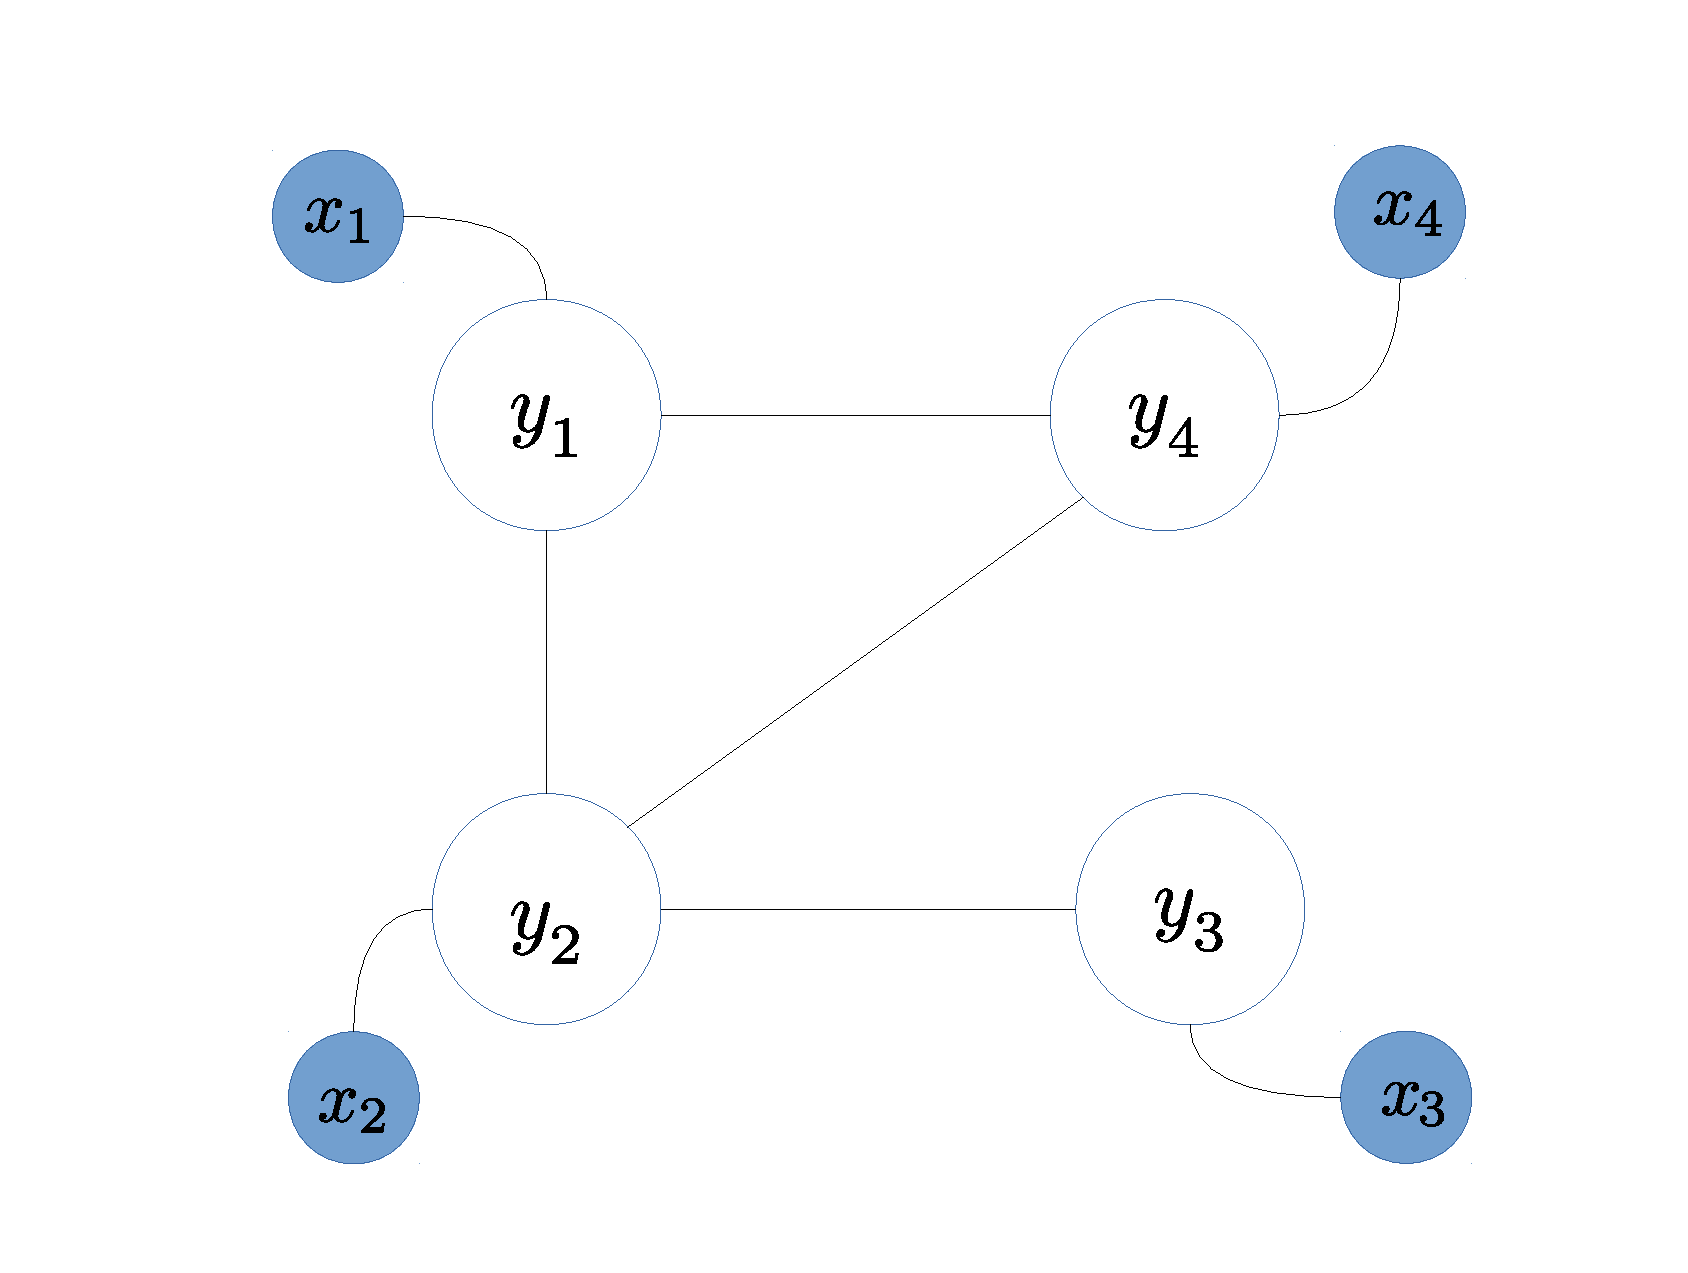
\includegraphics[height=8.5cm, width=11.5cm]{crf.eps}
		\caption{Simple example of conditional random field.}		
		\label{crf}
	\end{center}
\end{figure} 
According to Hammersley-Clifford theorem \cite{hammersley1968markov}, the the factors must be always positive, we can employ log-linear models for the potential functions, which results in:
\begin{equation}
\label{crf_potential}
\begin{aligned}
p(\bld y | \bld x; \bld \theta) &= \frac{1}{Z(\bld x, \bld \theta)}\prod_{c\in \mathcal{C}}\exp(\langle\phi(x_c, y_c), \bld \theta\rangle)\\
&=\frac{1}{Z(\bld x, \bld \theta)}\exp(\sum_{i\in V}\langle\phi_u(x_i, y_i), \bld{\theta}_u\rangle + \sum_{(i,j)\in \mathcal{E}}\langle\phi_p(x_i, x_j, y_i, y_j), \bld{\theta}_p\rangle)
\end{aligned}
\end{equation}
being $\langle \cdot, \cdot \rangle$ the inner product, and $\phi(x_c, y_c)$ the sufficient statistic of the factor over clique $c$. Because we consider the potentials up to second order, only feature function for unary potential $\phi_u(\cdot)$ and feature function for pairwise potential $\phi_p(\cdot)$ are considered here. This function can also be treated as feature function which extracts feature of the data over clique. 

Now we have made assumptions of graph structure and conditional dependency for the graph. This can be interpreted as a filter of a probability distribution family. Only the class of probability distribution that satisfies these assumptions such as up to second order potentials can be expressed and learned with this graph. To further identify different probability distribution in this class, we need to parameterize it and identify it with specific parameters which can learned during training. 

\paragraph{Parametrization} of the probability distribution is expressed explicitly in Eq.\ref{crf_potential}. This means that the dimension of the parameter in each kind of potential should be the same as the dimension of feature function. In this work, the feature function should be a function of input and class label, while the feature function can also be the function of only input and weight should be defined as matrix whose output dimension is the number of class serving as a linear mapping. In this work, we only consider the former case.

Regarding \textbf{unary feature}, we utilize the probability vector $p(y_i|x_i)$ which is predictive likelihood from a discriminative classifier which is a deep neural network in this work. 

\paragraph{Pairwise feature} in this work is quite simple context cue in the scene which is defined as binary co-occurrence matrix $\bld H(y_i,y_j)$. If one category occurs with another category in the same scene, then the corresponding entry in the matrix is filled with 1, otherwise 0. 

Although obtaining this pairwise feature requires knowing the ground truth labels of objects in the scene, it still makes sense in the application of this work. Because we use T-LESS dataset which will be introduced in the experiment part, each of scene images in this dataset contains multiple industrial-relevant texture-less objects, some of them are combination of objects of other categories. We want to simulate the situation that, we treat each scene as one product which is composed of multiple sub-parts. Because we know the product, and thus we also know the real labels of components of this product which is corresponding to the co-occurrence of objects in this scene and our goal is to classify the components with help of this contextual information.

Based on these two kinds of features, we have the formulation of likelihood function of CRF model for one scene as follows:
\begin{equation}
\label{crf_used}
p(\bld y|\bld x; \bld \theta) = \frac{1}{Z(\bld x, \bld \theta)}\exp(\theta_u\sum_{i\in V}p(y_i|x_i) + \theta_p\sum_{(i,j)\in \mathcal{E}}\bld H(y_i,y_j))
\end{equation}
where $\bld \theta = \{\theta_u, \theta_p\} \in \mathbb{R}^2$.

\section{Learning}
The most popular approach is estimate $\bld \theta$ is maximum likelihood estimate(MLE). The likelihood for one scene is defined in Eq.\ref{crf_used}. Normally we have large size of scenes in training set where each of them contains multiple objects. We denote training set by $\mathcal{D} = [d_1, ..., d_m]$, where each scene is represented by $d_i = (\bld x^i, \bld y^i)$. For each scene, we create a CRF model for it. Therefore we can denote the whole set of graph by $\bld{\mathcal{G}}=[\mathcal{G}_1, ..., \mathcal{G}_m]$, where $\mathcal{G}_i = (V_i, \mathcal{E}_i)$. This is consistent to previous notations when we make little modifications for $\bld x$ and $\bld y$: $\bld x^i = [x^i_1, ..., x^i_n,]$ and $\bld y^i = [y^i_1, ..., y^i_n]$. For computational convenience and stability, negative log likelihood as objective function is always employed. The objective in MLE on training set is defined as fallows:
\begin{equation}
\label{crf_obj}
\mathcal{NLL}(\bld \theta; \mathcal{D}) = -\sum_{i=1}^{m}\big(\theta_u\sum_{j\in V_i} p(y_j^i|x_j^i) + \theta_p\sum_{(j,k)\in\mathcal{E}_i}\bld H(y_j^i, y_k^i)  - Z_l(\bld x^i; \bld \theta)\big)
\end{equation}     
where 
\begin{equation}
\label{log_partition_func}
Z_l = \log
\big(
\sum_{\bld y^i \in \mathcal{Y}} 
\big( 
\theta_u\sum_{j\in V_i}p(y_j^i|x_j^i) + \theta_p\sum_{(j,k)\in \mathcal{E}_i}\bld H(y_j^i, y_k^i) 
\big) 
\big)
\end{equation}

With this expression, our problem is defined in the following form with MLE:
\begin{equation}
\label{crf_nll_opt}
\bld \theta^\star = \underset{{\bld \theta}}{argmin} \big[\mathcal{NLL(\bld \theta; \mathcal{D})}\big]
\end{equation}

The log likelihood function of CRF is proved to be concave \cite{koller2009probabilistic}, which means the local optimizer is also the global optimizer although it's not unique. To optimize this objective w.r.t. the model parameters on dataset with large size, we can employ stochastic gradient descent (SGD), which requires to calculate the gradient of object w.r.t. the model parameters $\bld \theta$. The gradients can be computed as follows, where we use $\bld \theta$ to represent parameters in order to make the expression clear:
\begin{equation}
\label{crf_grad}
\frac{\partial}{\partial \bld \theta} \mathcal{NLL}(\bld \theta; \mathcal{D}) = -\sum_{i=1}^{m}
\big(
\phi(\bld x^i, \bld y^i) - 
\mathbb{E}_{p(\bld y|\bld x^i;\bld \theta)}
\big[\phi(\bld x^i, \bld y)\big]
\big)
\end{equation}
where the expectation $\mathbb{E}_{p(\bld y|\bld x^i;\bld \theta)}
\big[\phi(\bld x^i, \bld y)\big]$ stands for the partial derivative of the log-partition function, which is retrieved by:
\begin{equation}
\label{exp_log_part}
\mathbb{E}_{p(\bld y|\bld x^i;\bld \theta)}
\big[\phi(\bld x^i, \bld y)\big] = \sum_{\bld y\in\mathcal{Y}}p(\bld y|\bld x^i;\bld \theta)\phi(\bld y, \bld x^i)
\end{equation}
The gradients of parameters corresponds to the difference between the empirical expectation of its associated sufficient statistics (the sufficient statistics of ground truth) and its expectation over the estimated probability distribution $p(\bld y|\bld x; \bld \theta)$. The goal of the optimization is to decrease the gradients until they reach zero, which means that we match of first moment of sufficient statistics over the output distribution. Therefore this way is also called moment matching.

When taking a closer look at Eq. \ref{crf_grad} and Eq. \ref{exp_log_part}, to calculate the gradients in each step of SGD, we need to compute $p(\bld y|\bld x; \bld \theta)$, which requires to compute the partition function $Z(\cdot)$. Because the number of possible assignments grows exponentially in the number of classes, it's infeasible to get a exact solution in practice. This problem also appears when we want to obtain a probability distribution(marginal inference) instead of a single prediction(MAP inference) in testing time. To compute the probability distribution in probabilistic modeling always refers to as inference. There are a bunch of research works focusing on inference. Because the CRF model in this work is fully connected, we adopt a popular and effective approach which is called loopy belief propagation and introduced in next subsection. This approach can provide a approximation to the log-partition function $Z_l(\cdot)$, which is required in \ref{exp_log_part} and to the marginal probability distribution of random variables in $\bld y$ to be plugged in \ref{crf_grad} in the graph with cycles and exact solution in graph without cycle.


\section{Inference}
Loopy belief propagation introduced by \cite{pearl2014probabilistic}, also known as sum-product algorithm, is a popular approach for probabilistic inference in graphical models. Briefly, this approach is based on the exchange of statistical information among the nodes in the graph according to their relationships. The core idea behind that is for each node in the graph to maintain its belief, which is a $k$-dimensional vector $\bld b(y_i)$ if the node is discrete random variable where $k$ is the number of class. The $i$-th entry of this vector indicates the probability that $i$-th class is assigned to this node. The belief of a node evolves as it receives \textit{messages} from it neighbors. A message $\bld m_{ij}(y_j)$ sent from node $y_i$ to node $y_j$ encodes belief of $y_i$ about what class node $y_j$ should belong to. This message, in turn, based on the messages it received from all the other neighbors except for the recipient in a previous time-step.

The algorithm keeps sending messages until the graph is calibrated, which means that the messages of two consecutive iterations are less than one threshold. However, in practice, the algorithm can not calibrate or converge. A maximum number of iteration can be set to obtain satisfactory results. The messages computation is as follows:
\begin{equation}
\label{message}
\bld m_{ij}(y_j) = \sum_{y_i\in \mathcal{Y}_i}\psi_{ij}(y_i, y_j, x_i, x_j, \theta_p)\psi_i(y_i, x_i, \theta_u) \prod_{y_k\in\mathcal{N}(y_i)\backslash y_j}\bld m_{ki}(y_i)
\end{equation}
where $\mathcal{N}(y_i) \backslash y_j$ is the set of node neighbors of $y_i$ except for $y_j$. Once the iteration reaches maximum number or the graph is calibrated, we can compute the belief of each node as follows:

\begin{equation}
\label{belief}
\bld b(y_i) = \frac{1}{Z_i}\psi_i(y_i, x_i, \theta_u) \prod_{y_j\in\mathcal{N}(y_i)}\bld m_{ji}(y_i)
\end{equation}
where $Z_i$ is the normalizer of unnormalized belief of node $y_i$ to ensure the sum of marginal probability of $y_i$ is 1. 

For the implementation, we employ the library in C++ from \cite{Ruiz-Sarmiento-REACTS-2015}. However, the weights in this library are assumed to be category-independent, which means that the weights are defined as weight matrix to build a linear mapping from feature function to potential function. Therefore we need to modify the type of weights in this library in order to incorporate different type of weight defined in Eq. \ref{crf_used}, which serve as coefficient of potential function instead of a linear mapping inside the potential function. To note that the messages are initialized uniformly during loopy belief propagation.


